\documentclass[brazil]{beamer}
\usepackage[utf8]{inputenc}
\usepackage[T1]{fontenc}
\usepackage{lmodern}
\usepackage{graphicx}			%para imagens
\usepackage{epstopdf} 			%resolve problemas eps-pdf
\usepackage{fancyhdr}			% para o cabeçalho bonito
\usepackage{caption}				%para legendas
\usepackage{placeins} 			%controlar o lugar dos floats
\usepackage{color}
\usepackage{url}
\usepackage{bm}
\renewcommand{\UrlFont}{\tiny}
\usepackage{relsize}
\usepackage{hyperref}

\usetheme{Dresden}
\usecolortheme{orchid}
\setbeamertemplate{navigation symbols}{}

\newcommand{\HRule}{\rule{\linewidth}{0.5mm}}

\title{Controle para Automação \\ Cadeias de Markov}
\author{Juarez Sampaio \\ Rodrigo}
\titlegraphic{\leavevmode\smash{\raisebox{5.5cm}{
\includegraphics[width=0.8\textwidth]{./img/logo.jpg}}}}
\institute{Universidade de Brasília}
\date{30 de Novembro de 2016}


\begin{document}
\begin{frame}
        \titlepage
\end{frame}

\begin{frame}[fragile]
  \frametitle{Conteúdo}
  \begin{itemize}
     \item Revisão e Notação de Probabilidade
     \item Introdução - Cadeias de Markov
     \item Problema
     \item Problema de Decisão de Markov
     \item Aplicações
  \end{itemize}
\end{frame}

\begin{frame}[fragile]
  \frametitle{Revisão Probabilidade}

  \begin{itemize}
      \item Probabilidade Conjunta: 
        $$ P (A, B)$$ 
      \item Probabilidade Condicional: 
        $$P ( A | B ) = \frac{P(A,B)}{P(B)}$$
      \item Probabilidade Total:
      sejam eventos $B_i$ mutualmente excludentes ($B_i \cap B_j = \varnothing$,
      )se $i \neq j$ e tais que $\cup _i B_i = \Omega_i$:
      $$ P[A] = \sum_i P[A | B_i] P[B_i]$$
      \item Regra de Bayes

        $$P[B_k | A] = \frac{P[A | B_k] P[B_k]}{\sum_i P[A | B_i] P[B_i]}$$
  \end{itemize}

\end{frame}
\begin{frame}
  \frametitle{AFD}
      \begin{figure}
        \centering
        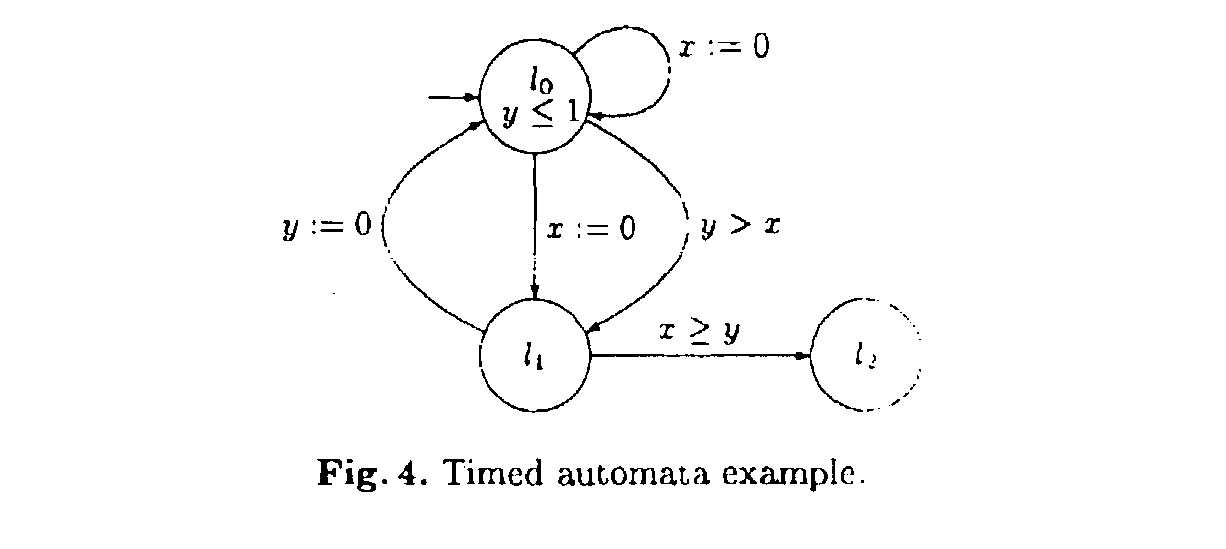
\includegraphics[width = 1.0\textwidth, keepaspectratio]{./img/automata.png}
        \caption{AFD. Semelhança: estados e transições. Diferença: eventos são
          substituídos por probabilidade de ocorrência da transição.
          \cite{sample} }
      \end{figure}
\end{frame}

\begin{frame}
    {\footnotesize
    \bibliographystyle{abnt-num}
    \bibliography{apresentacao}
    }
\end{frame}


\end{document}
